\chapter{Specifications}
\label{app:RunSpec}

\section{Summary of enzyme types}

\begin{table}[htbp!]
    \caption{Summary of all the enzyme types that are referenced in this work. It is important to mention, that, for reasons of comprehensiveness, this table exemplarily only includes the rules which are in favour of acetylation (i.e. acetylation adders and methylation removers). However, every enzyme set used in this work is completely symmetrical. This means that if an enzyme set contains a linear acetylation adder it also contains a linear methylation adder at equal association and dissociation rates respectively and so forth.}
    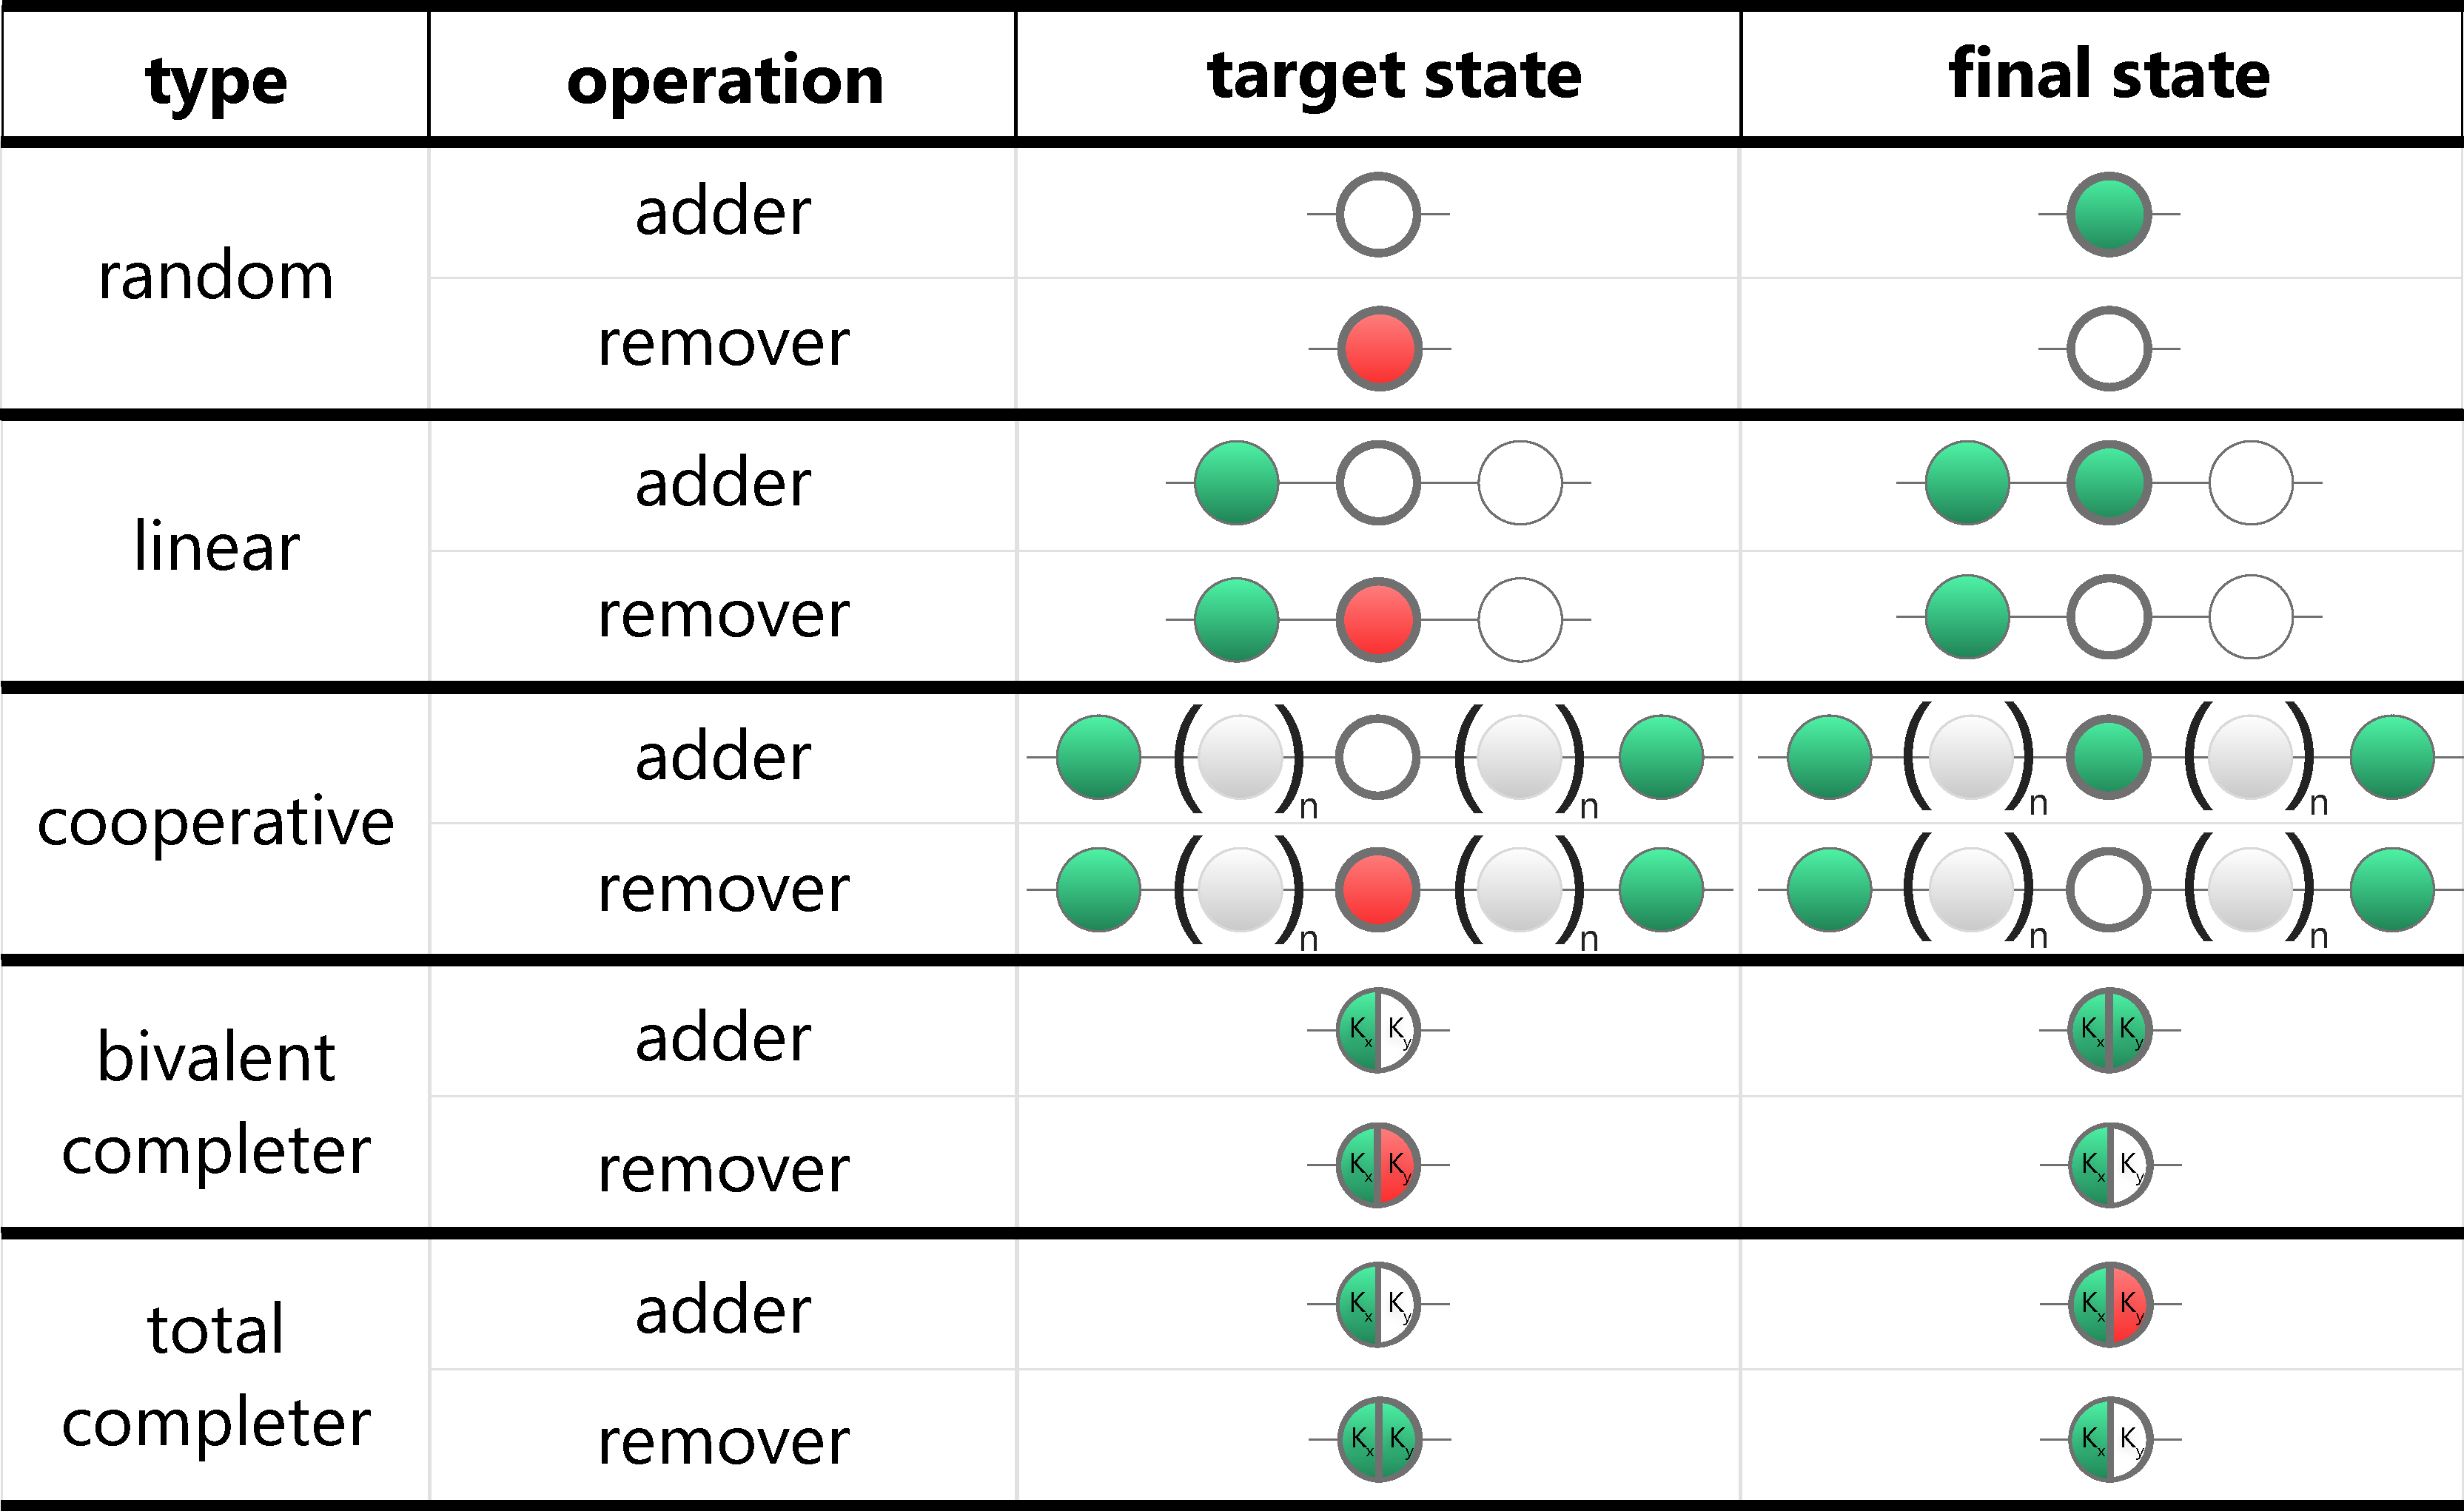
\includegraphics[width=\textwidth]{enzymes/table.pdf}
    \label{img:enzymeTypeSummary}
\end{table}

\section{Summary of simulation parameters}

\begin{table}[htbp!]
    \caption{Summary of the simulation parameters explained in \ref{sec:simulationDetails} sorted by subsections in the 'Results' section.}
    \centering
    \begin{tabular}{lllllrr}
                                &   &                               & coop?          & cyclic? & \multicolumn{1}{l}{diss?} & \multicolumn{1}{l}{simulation time}  \\
        \multicolumn{1}{r}{3.1} & ~ & long                          & no coop        & no      & 100000                    & 5                                    \\
        ~                       & ~ & short                         & no coop        & no      & 100000                    & 1                                    \\
        \multicolumn{1}{r}{3.2} & ~ & long                          & no coopRem     & no      & 100000                    & 5                                    \\
        ~                       & ~ & long                          & w coopRem      & no      & 100000                    & 5                                    \\
        ~                       & ~ & short                         & no coopRem     & no      & 100000                    & 1                                    \\
        ~                       & ~ & short                         & w coopRem      & no      & 100000                    & 1                                    \\
        \multicolumn{1}{r}{3.3} & ~ & long                          & no coopRem     & yes     & 100000                    & 20                                   \\
        ~                       & ~ & long                          & w coopRem      & yes     & 100000                    & 20                                   \\
        ~                       & ~ & short                         & no coopRem     & yes     & 100000                    & 8                                    \\
        ~                       & ~ & short                         & w coopRem      & yes     & 100000                    & 8                                    \\
        \multicolumn{1}{r}{3.4} & ~ & long                          & no coopRem     & yes     & 100000                    & 20                                   \\
        ~                       & ~ & long                          & no coopRem     & yes     & 100                       & 20                                   \\
        ~                       & ~ & short                         & no coopRem     & yes     & 100000                    & 6                                    \\
        ~                       & ~ & short                         & no coopRem     & yes     & 100                       & 6                                    \\
        \multicolumn{1}{r}{3.5} & ~ & maxReach0 (long)              & no coopRem     & yes     & 100000                    & 20                                   \\
        ~                       & ~ & maxReach1                     & no coopRem     & yes     & 100000                    & 20                                   \\
        ~                       & ~ & maxReach2                     & no coopRem     & yes     & 100000                    & 20                                   \\
        ~                       & ~ & maxReach3                     & no coopRem     & yes     & 100000                    & 20                                   \\
        ~                       & ~ & maxReach4                     & no coopRem     & yes     & 100000                    & 20                                   \\
        ~                       & ~ & maxReach5                     & no coopRem     & yes     & 100000                    & 20                                   \\
        ~                       & ~ & maxReach6                     & no coopRem     & yes     & 100000                    & 20                                   \\
        \multicolumn{1}{r}{3.6} & ~ & BivalentBistability
          (short) & no coopRem 2 K & yes     & 100000                    & 10                                   \\
        ~                       & ~ & FavBivalency (short)          & w coopRem      & yes     & 10000                     & 2                                    \\
        ~                       & ~ & FavTotal (short)              & w coopRem      & yes     & 10000                     & 2
    \end{tabular}
    \label{tab:simulationParametersSummary}
\end{table}
\begin{itemize}
    {
        \color{red}
        \item Explain coop?
        \item Decide on whether to insert cyclic?
        \item Add subsubsections to table
    }
\end{itemize}



